\documentclass[]{article}
\usepackage{lmodern}
\usepackage{amssymb,amsmath}
\usepackage{ifxetex,ifluatex}
\usepackage{fixltx2e} % provides \textsubscript
\ifnum 0\ifxetex 1\fi\ifluatex 1\fi=0 % if pdftex
  \usepackage[T1]{fontenc}
  \usepackage[utf8]{inputenc}
\else % if luatex or xelatex
  \ifxetex
    \usepackage{mathspec}
  \else
    \usepackage{fontspec}
  \fi
  \defaultfontfeatures{Ligatures=TeX,Scale=MatchLowercase}
\fi
% use upquote if available, for straight quotes in verbatim environments
\IfFileExists{upquote.sty}{\usepackage{upquote}}{}
% use microtype if available
\IfFileExists{microtype.sty}{%
\usepackage{microtype}
\UseMicrotypeSet[protrusion]{basicmath} % disable protrusion for tt fonts
}{}
\usepackage[margin=1in]{geometry}
\usepackage{hyperref}
\hypersetup{unicode=true,
            pdfborder={0 0 0},
            breaklinks=true}
\urlstyle{same}  % don't use monospace font for urls
\usepackage{natbib}
\bibliographystyle{plainnat}
\usepackage{longtable,booktabs}
\usepackage{graphicx,grffile}
\makeatletter
\def\maxwidth{\ifdim\Gin@nat@width>\linewidth\linewidth\else\Gin@nat@width\fi}
\def\maxheight{\ifdim\Gin@nat@height>\textheight\textheight\else\Gin@nat@height\fi}
\makeatother
% Scale images if necessary, so that they will not overflow the page
% margins by default, and it is still possible to overwrite the defaults
% using explicit options in \includegraphics[width, height, ...]{}
\setkeys{Gin}{width=\maxwidth,height=\maxheight,keepaspectratio}
\IfFileExists{parskip.sty}{%
\usepackage{parskip}
}{% else
\setlength{\parindent}{0pt}
\setlength{\parskip}{6pt plus 2pt minus 1pt}
}
\setlength{\emergencystretch}{3em}  % prevent overfull lines
\providecommand{\tightlist}{%
  \setlength{\itemsep}{0pt}\setlength{\parskip}{0pt}}
\setcounter{secnumdepth}{5}
% Redefines (sub)paragraphs to behave more like sections
\ifx\paragraph\undefined\else
\let\oldparagraph\paragraph
\renewcommand{\paragraph}[1]{\oldparagraph{#1}\mbox{}}
\fi
\ifx\subparagraph\undefined\else
\let\oldsubparagraph\subparagraph
\renewcommand{\subparagraph}[1]{\oldsubparagraph{#1}\mbox{}}
\fi

%%% Use protect on footnotes to avoid problems with footnotes in titles
\let\rmarkdownfootnote\footnote%
\def\footnote{\protect\rmarkdownfootnote}

%%% Change title format to be more compact
\usepackage{titling}

% Create subtitle command for use in maketitle
\newcommand{\subtitle}[1]{
  \posttitle{
    \begin{center}\large#1\end{center}
    }
}

\setlength{\droptitle}{-2em}
  \title{}
  \pretitle{\vspace{\droptitle}}
  \posttitle{}
  \author{}
  \preauthor{}\postauthor{}
  \date{}
  \predate{}\postdate{}

\usepackage{booktabs}
\usepackage{amsthm}
\makeatletter
\def\thm@space@setup{%
  \thm@preskip=8pt plus 2pt minus 4pt
  \thm@postskip=\thm@preskip
}
\usepackage{xcolor}
\usepackage{float}
\usepackage[utf8]{inputenc}
\usepackage[brazil]{babel}
\usepackage{colortbl}
\usepackage{tikz}

\usepackage{amsthm}
\newtheorem{theorem}{Teorema}[section]
\newtheorem{lemma}{Lema}[section]
\theoremstyle{definition}
\newtheorem{definition}{DEF}[section]
\newtheorem{corollary}{Corolário}[section]
\newtheorem{proposition}{Proposição}[section]
\theoremstyle{definition}
\newtheorem{example}{Exemplo}[section]
\theoremstyle{definition}
\newtheorem{exercise}{Exercise}[section]
\theoremstyle{remark}
\newtheorem*{remark}{Remark}
\newtheorem*{solution}{Solution}
\let\BeginKnitrBlock\begin \let\EndKnitrBlock\end
\begin{document}

\begin{titlepage}
\centering{\large{UNIVERSIDADE FEDERAL DO PARANÁ}}
\\
\centering{Departamento de Estatística}

\vspace{7.5cm}

\centering{\huge{CE222 - Processos Estocásticos}}

Prof. Benito Orlando Olivares Aguilera

\vspace{2cm}


Andryas Waurzenczak

\vfill

2018-05-08
\end{titlepage}

{
\setcounter{tocdepth}{2}
\tableofcontents
}

\newpage

\section*{Introdução}\label{introducao}
\addcontentsline{toc}{section}{Introdução}

O objetivo dessa página é guardar as anotações, atividades e trabalhos
da disciplina CE222 - Processos Estocásticos Aplicados, ministrada pelo
Professor \href{https://docs.ufpr.br/~benitoag/}{Benito Olivares
Aguilera}.

\subsection*{Processos Estocásticos
Aplicados}\label{processos-estocasticos-aplicados}
\addcontentsline{toc}{subsection}{Processos Estocásticos Aplicados}

Objetivo da disciplina: Possibilitar ao aluno a aplicação de técnicas de
processos estocásticos na análise de problemas de diversas áreas.

\subsubsection*{EMENTA}\label{ementa}
\addcontentsline{toc}{subsubsection}{EMENTA}

A ementa da disciplina está dividida em duas partes. A primeira parte
referente a teoria básica de processos. A segunda parte é o
desenvolvimente da parte teórica em diversas aplicações.

\subsubsection*{Parte I - Teórica}\label{parte-i---teorica}
\addcontentsline{toc}{subsubsection}{Parte I - Teórica}

\begin{enumerate}
\def\labelenumi{\arabic{enumi}.}
\tightlist
\item
  PROCESSOS ESTOCÁSTICOS: Introdução. Teoria básica de processos.
  Classificação de processos. Processos Estacionários. Seqüências
  Independentes. Passeio Aleatório. Ruína do Jogador. Sistemas Lineares.
\item
  PROCESSOS DE SEGUNDA ORDEM: Função Média, Variância e Covariância.
  Processos Fracamente Estacionários.
\item
  CADEIAS DE MARKOV: Cadeias Markovianas de Parâmetro Discreto. Cadeias
  Markovianas de Parâmetro Contínuo. O Processo de Nascimento e Morte.
  Processo de Poisson. Introdução à Teoria das Filas.
\item
  PROCESSOS GAUSSIANOS: O Processo de Wiener.
\end{enumerate}

\subsubsection*{Parte II - Prática}\label{parte-ii---pratica}
\addcontentsline{toc}{subsubsection}{Parte II - Prática}

\begin{enumerate}
\def\labelenumi{\arabic{enumi}.}
\setcounter{enumi}{4}
\tightlist
\item
  Aplicações de Cadeias de Markov
\item
  Teoria de Filas
\item
  Sistemas lineares e controle.
\end{enumerate}

Link para
\href{https://docs.ufpr.br/~benitoag/ce222-2018.html}{disciplina}

\section{Revisão}\label{revisao}

\subsection{Fenômenos}\label{fenomenos}

Fenômenos são acontecimentos observáveis. Tem-se dois tipos de
fenômenos:

\begin{itemize}
\tightlist
\item
  Determinístico
\end{itemize}

Sob certas condições de regularidade, o resultado, é previsível.

Ex: Ferver água, por exemplo, sabe-se que quando aquecida a 100ºC, sobre
pressão normal, entre em ebulição.

\begin{itemize}
\tightlist
\item
  Aleátorio
\end{itemize}

Os resultados são imprevisíveis.

Ex: Lançamento de um dado, não sabemos que número vai sair.

Aqui, neste curso de processos estocásticos estaremos interessandos no
segundo tipo de evento (aleátorio), onde por meio de probabilidade
podemos ter uma ideia do comportamento/resultado futuro.

\begin{quote}
A seguir algumas definições de probabilidade que serão utilizadas ao
decorrer do curso.
\end{quote}

\subsection{Definições de
Probabilidade}\label{definicoes-de-probabilidade}

\BeginKnitrBlock{definition}
\protect\hypertarget{def:probabilidade}{}{\label{def:probabilidade} }Dado um
experimento aleátorio \(\varepsilon\), chamamos de espaço amostral o
conjunto (não vazio) de \textbf{todos} os resultados possíveis
(\(\Omega\)). O conjunto de todos os objetos aos quais poderemos
atribuir uma probabilidade é chamado de \(\sigma\)-álgebra. No caso do
\(\Omega\) finito (ou enumerável) a sigma-álgebra será o conjunto das
partes de \(\Omega\) (Conjunto potência).
\EndKnitrBlock{definition}\\
\BeginKnitrBlock{example}
\protect\hypertarget{exm:unnamed-chunk-1}{}{\label{exm:unnamed-chunk-1}
}Lançamento de uma moeda uma vez.\\
A = P(\(\Omega\)) = (\{c\},\{k\}, \(\Omega\), \(\phi\))
\EndKnitrBlock{example}\\
\BeginKnitrBlock{example}
\protect\hypertarget{exm:unnamed-chunk-2}{}{\label{exm:unnamed-chunk-2}
}Lançamento de um dado.\\
F = P(\(\Omega\)) = \{\{1\},\{2\},\ldots{},\{1,2\},\{1,3\},
\ldots{},\{1,2,3\},\ldots{},\(\Omega\),\(\phi\)\}
\EndKnitrBlock{example}\\
Para intervalos contínuos \(\sigma\)-álgebra de Bórel.

F = \(\beta_{[0,1)}\) =\textgreater{} \(\sigma\)-álgebra de Bórel

\BeginKnitrBlock{definition}[Definição Clássica]
\protect\hypertarget{def:unnamed-chunk-3}{}{\label{def:unnamed-chunk-3}
\iffalse (Definição Clássica) \fi{} } P(A) = \(\frac{\#A}{\#\Omega}\)\\
Utiliza-se quando os pontos são equiprovaveis.
\EndKnitrBlock{definition}\\
\BeginKnitrBlock{definition}[Definição Geométrica]
\protect\hypertarget{def:unnamed-chunk-4}{}{\label{def:unnamed-chunk-4}
\iffalse (Definição Geométrica) \fi{} }P(A) =
\(\frac{compr(A)}{compr(\Omega)}\)
\EndKnitrBlock{definition}\\
\BeginKnitrBlock{definition}[Definição Frequentista]
\protect\hypertarget{def:unnamed-chunk-5}{}{\label{def:unnamed-chunk-5}
\iffalse (Definição Frequentista) \fi{} }P(A) = \(\frac{A}{N}\)
\EndKnitrBlock{definition}\\
\BeginKnitrBlock{definition}[Definição de Probabilidade]
\protect\hypertarget{def:unnamed-chunk-6}{}{\label{def:unnamed-chunk-6}
\iffalse (Definição de Probabilidade) \fi{} }Uma medidade de
probabilidade P como uma função de \(\Omega\) em \(\mathbb{R}\) tal que:

\begin{itemize}
\tightlist
\item
  P(A) \(\leq\) 0, \(\forall\) A \(\in\) F (existe um evento pelo menos)
\item
  P(\(\Omega\)) = 1
\item
  P(\(\cup_i A_i\)) = \(\sum_i P(A_i)\), se os Ai's são dijuntos
\end{itemize}
\EndKnitrBlock{definition}\\
\BeginKnitrBlock{definition}[Espaço de Probabilidade]
\protect\hypertarget{def:unnamed-chunk-7}{}{\label{def:unnamed-chunk-7}
\iffalse (Espaço de Probabilidade) \fi{} }(\(\Omega\),F,P)

Um espaço de probabilidade como o trio (\(\Omega\),F,P) - (Espaço
amostral, \(\sigma\)-álgebra, medidade de probabilidade)
\EndKnitrBlock{definition}\\
\BeginKnitrBlock{definition}[Probabilidade Condicional]
\protect\hypertarget{def:unnamed-chunk-8}{}{\label{def:unnamed-chunk-8}
\iffalse (Probabilidade Condicional) \fi{} }Dados A e B \(\in\) F:
P(A\textbar{}B) = \frac{P(A \cap B)}{P(B)}, P(B) \textgreater{} 0

Para duas variáveis aleátorias X, Y \(\in\) (\(\Omega,F,P\))

\[P(X \in B_1 | Y \in B_2) = \frac{P(X \in B_1,Y \in B_2)}{P(Y \in
B_2)}\]

para \(B_1\), \(B_2\) bolineanos e P(Y \(\in\) \(B_2\)) \textgreater{}
0.
\EndKnitrBlock{definition}\\
\BeginKnitrBlock{example}[Exemplo de Probabilidade Condicional]
\protect\hypertarget{exm:unnamed-chunk-9}{}{\label{exm:unnamed-chunk-9}
\iffalse (Exemplo de Probabilidade Condicional) \fi{} }Sejam X e Y va's
no mesmo espaço parâmetrico. Tais que
X\textasciitilde{}Poi(\(\lambda_1\)) e
Y\textasciitilde{}Poi(\(\lambda_2\)). Defini-se Z = X + Y. Encontrar a
distribuição de X\textbar{}Z, sabendo que X é independente de Y.

\[P(X $\in$ B_1| Z \in B_2$)\]

Como X e Y são discretas, podemos considerar somente os bolineanos
\(B_1\)= \{x\} e \(B_2\) = \{z\} temos assim:

P(X = x\textbar{}Z=z) = P(X=x\textbar{}X+Y=z) =
\(\frac{P(X=x,X+Y==z)}{P(X+Y=z)}\) = \(\frac{P(X=x,Y=z-x)}{P(X+Y=z)}\) =
\(\frac{P(X=x)P(Y=z-x)}{P(X+Y=z)}\)

Sabemos que se X \textasciitilde{} Poi(\(\lambda_1\)) e Y
\textasciitilde{} Poi(\(\lambda_2\)), X independente de Y, então X + Y
\textasciitilde{} Poi (\(\lambda_1 + \lambda_2\)).

P(X=x\textbar{}X + Y =z) =
\(\large \frac{\frac{e^{-\lambda x} \lambda_1^x}{x!} \frac{e^{-\lambda_2 } \lambda_2^{z-x}}{(z-x)!}}{\frac{e^{-(\lambda_1 + \lambda_2)z} (\lambda_1 + \lambda_2)^z}{z!}} = \frac{z! \lambda_1^x \lambda_2^{z-x}}{x!(z-x)! \frac{(\lambda_1 + \lambda_2)^z}{(\lambda_1 + \lambda_2)^x (\lambda_1 + \lambda_2)^{z-x}}} = \binom{z}{x} \binom{\lambda_1}{\lambda_1 + \lambda_2}^x \binom{\lambda_2}{\lambda_1 + \lambda_2}^{z-x}\)

Temos então:

\[X|X+Y = z \sim Bin(z,\frac{\lambda_1}{\lambda_1 + \lambda_2})\]
\EndKnitrBlock{example}

\section{Processo Estocástico}\label{processo-estocastico}

\subsection{O que é um Processo?}\label{o-que-e-um-processo}

Processo é um termo que indica a ação de avançar, de ir para frente. É
um conjunto sequencial de ações com objetivo comum.

Exemplos são: fabricas que produzem coca-cola por exemplo, onde existe
esteiras que vão levando latas de aluminio, que são pintadas,
preenchidas com liquido, lacradas, pressurizadas etc\ldots{}

\subsection{Processos Estocásticos}\label{processos-estocasticos}

\BeginKnitrBlock{definition}
\protect\hypertarget{def:unnamed-chunk-10}{}{\label{def:unnamed-chunk-10}
}Um processo estocástico é uma familia de variáveis aleátorias indexadas
por um conjunto T \(\neq\) \(\phi\).
\EndKnitrBlock{definition}

\[{X(t), t \in T} \text{ ou } {X_t, t \in T}\]

\(t_{fixo} \rightarrow\) va X(t)

\(w_{fixo} \rightarrow\) função real (chamada tragetoria do processo)

O conjunto de todas as trágetorias é chamado ``ensemble''.

A descrição completa de um processo estocástico pode ser extremamente
complexo, mas em certos processos uma estrutura de probabilidade
adequada pode facilitar tal descrição.

O conjunto T será chamado de \texttt{espaço\ de\ parâmetros}. Geralmente
o índice t será identificado como `tempo'. O conjunto S no qual a va
assume valores será chamado \texttt{espaço\ de\ estados}.

\BeginKnitrBlock{example}
\protect\hypertarget{exm:unnamed-chunk-11}{}{\label{exm:unnamed-chunk-11}
}No experimento do lançamento da moeda.\\
\{\(X_n\), n=1,\ldots{},24\}, sendo \(X_n\) uma va dicotômica em que S =
\{-1,1\}, T = \{1,2,\ldots{},24\}

Também definimos o processo \{\(G_n\),n=0,\ldots{},24\}.

Logo o resultado teriamos então.

T = \{0,1,2,\ldots{},24\} e S = \{-20,-19,\ldots{},0,1,\ldots{}28\}

Notar que na verdade, por se tratar de uma va existe uma dependência com
o espaço amostral \(\Omega\), isto é, deveriamos escrever X(w,n), mas
por simplicidade vamos escrever apenas X(n) ou \(X_n\).
\EndKnitrBlock{example}

\subsection{Espaços T e S}\label{espacos-t-e-s}

Dependendo da natureza dos espaços T e S temos, quatro casos a saber:

\subsubsection{T discreto e S discreto}\label{t-discreto-e-s-discreto}

Temos um PE discreto a tempo discreto

\BeginKnitrBlock{example}
\protect\hypertarget{exm:unnamed-chunk-12}{}{\label{exm:unnamed-chunk-12}
}Exemplo da moeda

\{Gn, n \(\in\) T\} sendo T = \{0,1,2,\ldots{},24\} e S =
\{-20,\ldots{},28\}
\EndKnitrBlock{example}

\subsubsection{T é contínuo e S
discreto}\label{t-e-continuo-e-s-discreto}

Temos um PE discreto e o tempo contínuo.

\BeginKnitrBlock{example}
\protect\hypertarget{exm:unnamed-chunk-13}{}{\label{exm:unnamed-chunk-13}
}\{\(X_t\), t \(\in\) T\} onde \(X_t\) nº de carros que passaram num
pedagio até o instante t.

T = {[}0, +\(\infty\){]}

S = \{0,1,2,3,4,\ldots{}.\}
\EndKnitrBlock{example}

\subsubsection{T discreto e S contínuo}\label{t-discreto-e-s-continuo}

Temos um PE contínuo e o tempo discreto.

\BeginKnitrBlock{example}
\protect\hypertarget{exm:unnamed-chunk-14}{}{\label{exm:unnamed-chunk-14}
}\{\(X_t\), t \(\in\) T\} A pressão diastolica de n-eisimo individuo.

T: \{1,2,3,\ldots{},N\} S: \{0,+\(\infty\)\}
\EndKnitrBlock{example}

\subsubsection{T contínuo e S contínuo}\label{t-continuo-e-s-continuo}

Temos um PE contínuo a tempo contínuo

\BeginKnitrBlock{example}
\protect\hypertarget{exm:unnamed-chunk-15}{}{\label{exm:unnamed-chunk-15}
}\{\(X_t\), t \(\in\) T\} voltagem na rede no instante t

T = (0,+\(\infty\))

S = (0,+\(\infty\))
\EndKnitrBlock{example}

\subsection{Descrição probabilística}\label{descricao-probabilistica}

Considere um PE \{\(X_t\), t \(\in\) T\}. Para \(t_1\) fixo, X(\(t_1\))
é uma va com função distribuição.

\[F_x(x_1,t_1) = P(X(t_1) \leq x_1) \rightarrow \text{  distribuicao de 1
ordem de X(t)}\]

Para \(t_1\) e \(t_2\) fixos, temos que:

\[F_x(x_1,x_2;t_1,t_2) = P(X(t_1) \leq x_1, x(t_2) \leq x_2) \rightarrow
\text{  distribuicao de 2 ordem de X(t)}\]

Em geral,

\[F_x(x_1,x_2,...,x_n;t_1,t_2,...,t_n) = P(X(t_1) \leq x_1, X(t_2) \leq
x_2, ..., X(t_n) \leq x_n)\]

\(X(t_1) \in (-\infty,x_1], X(t_2) \in (\infty,x_2],...\)

Distribuição da n-esima ordem de X(t).

Se as va's X(\(t_i\)) com i = 1,\ldots{},\(\mu\) fossem discretas,
podemos escrever:

\(P_x(x_1,x_2,...,x_n;t_1,...,t_n) = P(X(t_1)=x_1,...,X(t_n)=x_n)\)

\begin{itemize}
\tightlist
\item
  Se \(X(t)\) é um PE a tempo continuo podemos escrever:
\end{itemize}

\(f_x(x_1,...,x_n;t_1,...,t_n) = \frac{\partial^n F_x}{\partial x_1,...,\partial x_n}\)

A descrição completa precisaria calcular todas as distribuições de X
(distribuições-finita-dimensionalidades) o que seria muito dificil.
Felizmente, em determinados casos, é necessário calcular a penas as duas
primeiras distribuições ??? (momentos).

\subsection{Média, variância e
covariância}\label{media-variancia-e-covariancia}

\BeginKnitrBlock{definition}
\protect\hypertarget{def:funmed}{}{\label{def:funmed} }A função média de um
PE \{X(t), t \(\in\) T\}:

\[\mu_x(t)=E[X(t)]\]
\EndKnitrBlock{definition}\\
\BeginKnitrBlock{definition}
\protect\hypertarget{def:funvar}{}{\label{def:funvar} }A função variância do
processo X:

\[\sigma^2_x(t) = var[X(t)]\]
\EndKnitrBlock{definition}\\
\BeginKnitrBlock{definition}
\protect\hypertarget{def:funcov}{}{\label{def:funcov} }A função covariância
do PE X = \{X(t),t \(\in\) T\}:

\[K_x(s,t) = cov[X(s),X(t)] = E[X(s),X(t)] - \mu_x(s) \mu_x(t)\]
\EndKnitrBlock{definition}\\
\BeginKnitrBlock{definition}
\protect\hypertarget{def:funaut}{}{\label{def:funaut} }A função de
autocorrelação:

\[R_x(s,t)=E[X(s),X(t)] - \mu_x(s) \mu_x(t)\]
\EndKnitrBlock{definition}\\
\BeginKnitrBlock{example}
\protect\hypertarget{exm:unnamed-chunk-16}{}{\label{exm:unnamed-chunk-16}
}Seja o PE X(t) = \(Z_1\) + \(Z_2\) sendo \(Z_1\), \(Z_2\) iid N(0,1)

\begin{equation}
\begin{split}
\mu_x(t)  &= E[X(t)]\\
&= E[Z_1 cos \lambda t + Z_2 sen \lambda t]\\
&= \underbrace{E[Z_1]}_0 cos \lambda t + E[Z_2] sen \lambda t \\
&=0
\end{split}
\end{equation}

\\

\begin{equation}
\begin{split}
K_x(s,t)=cov[X(s),X(t)] &= cov[{Z_1 cos \lambda s + Z_2 sen \lambda s},
{Z_1 cos \lambda t + Z_2 sen \lambda t}] \\
&= cov(Z_1 cos \lambda s, Z_1 cos \lambda t) + cov(Z_1 cos \lambda s, Z_2
sen \lambda t) + \\ & cov(Z_2 sen \lambda s, Z_1 cos \lambda t) + cov(Z_2 sen
\lambda s, Z_2 sen \lambda t) \\
&= cos \lambda s . cos \lambda t . cov(Z_1,Z_2) + cov \lambda s. sen
\lambda t . cov(Z_1,Z_2) + \\& sen \lambda s . cos \lambda t
. cov(Z_2,Z_1) + sen \lambda s . sen \lambda t . cov(Z_2,Z_2)\\
&= cos \lambda s . cos \lambda t + sen \lambda s . sen \lambda t \\
&= cos(\lambda s - \lambda t)\\
&= cos[\lambda(s-t)]
\end{split}
\end{equation}
\EndKnitrBlock{example}

\section{Classificação de Processos}\label{classificacao-de-processos}

\subsection{Processos estacionários}\label{processos-estacionarios}

Um PE \{X(t), t \(\in\) T\} é chamado estacionário (ou estritamente
estacionário) se, \textbf{para todo n} e para qualquer conjunto de
tempos \(t_i\), \(t_i\) \(\in\) T(i = 1,2,\ldots{},n) tem-se que:

\[F_X(x_1,...,x_n;t_1,...,t_n) = F_X(x_1,...,x_n; t_1 + \pi,..., t_n +
\pi)\]

(distribuição da n-esima ordem)

Isso significa que a distribuição não é afetada por deslocamento no
tempo e X(t) e X(\(t+\pi\)) terão a mesma distribuição.

\begin{itemize}
\tightlist
\item
  Para a distribuição de 1º ordem temos que:
\end{itemize}

\[F_X(x;t) = F_X(x;t \pi) = F_X(x)\]

\(\mu_x(t) = \mu \text{ constante}\)

\(\sigma^2_x(t) = \sigma^2\)

Para ser estacionário é necessário ter média e variância constante, mas
não suficiente.

\subsection{Processos fracamente
estacinário}\label{processos-fracamente-estacinario}

Se a condição de estacionaridade é satisfeita somente para n \(\leq\) k
(até certa ordem) então diremos que o processo é fracamente
estacionário.

Se X(t) é estacionário de 2º ordem, ele é chamado de fracamente
estacionário (de 2º ordem). Ou, como outros autores colocam, processos
estacináriode ordem k.

\BeginKnitrBlock{theorem}
\protect\hypertarget{thm:unnamed-chunk-17}{}{\label{thm:unnamed-chunk-17}
}Um PE \{X(t), t \(\in\) T\} será fracamente estacionário se:

\begin{enumerate}
\def\labelenumi{\roman{enumi}.}
\tightlist
\item
  \(\mu_x(t) = \mu \text{ constante}\)
\item
  \(K_x(s,t) = K_x(|s-t|)\)

  \EndKnitrBlock{theorem}
\end{enumerate}

ou seja, a covariância depende somente da diferença entre \textbf{s} e
\textbf{t}.

\BeginKnitrBlock{example}
\protect\hypertarget{exm:unnamed-chunk-18}{}{\label{exm:unnamed-chunk-18}
}X(t) = \(Z_1 cos \lambda t + Z_2 sen \lambda t\) \(\mu_x(t) = 0\)
\(K_x(s,t) = cos[\lambda(s-t)]\)
\EndKnitrBlock{example}

OBS: Todo processo estritamente estacinário é também fracamente
estacinário, a recíproca, em geral, não é verdadeira.

\subsection{Processos independentes}\label{processos-independentes}

Um PE \{X(t, t \(in\) T)\} será chamado independente se para \(t_i\)
\(\in\) T, n = 2,3,\ldots{}

\[F_X(x_1,x_2,...,x_n; t_1,...,t_n) = \prod^n_{i=1} F_x(x_i;t_i)\]

Nesse caso uma distribuição de primeira, será suficiente para
caracterizar o processo.

\subsection{Processos, com incrementos independentes e
estacionários}\label{processos-com-incrementos-independentes-e-estacionarios}

Um processo \{X(t), t \(\in\) T\} terá incrementos independentes se,
para t 0 \textless{} \(t_1 < t_2 < ... < t_n\) as va's
\(X(0),X(t_1) - X(0), X(t_2)-X(t_1),..., X(t_n) - X(t_{n-1})\) são
independentes.

Isto é, o número de ocorrências de X(t) em intervalos disjuntos de tempo
são variáveis independentes.

Se X(t) possui incrementos independentes e ainda X(t) - X(s) tem a mesma
distribuição que X(t+ \(\pi\)) - X(s + \(\pi\)) ,
\(\forall s,t,\pi >0\), s \textless{} t diremos que o processo possui
incrementos independentes estacionários.

\section{Cadeias de Markov}\label{cadeias-de-markov}

Diremos que um PE \{X(t), t \(\in\) T\} satisfaz a propriedade
markoviana (PM) se:

\[P(X(t_{n+1}) \leq | X(t_1) = x_1,...,X(t_n)=x_n) = P(X(t_{n+1}) \leq
X_{n+1} | X(t_n) = x_n)\]

Isso significa que a probabilidade condicional não leva em consideração
o que ocorreu antes do instante \(t_n\) para calcular a probabilidade no
instante \(t_n + 1\)\_

\subsection{Caso particular}\label{caso-particular}

No caso particular em que as VA's X(t) são DISCRETAS a propriedade
markoviana (PM) fica:

\[P(\underbrace{X_{n+1}}_{\text{Variável aleátoria}} =
\underbrace{x_{n+1}}_{\text{número real}}| X_1 = x_1,...,X_n=x_n) =
P(X_{n+1} = X_{n+1}| X_n = x_n)\]

Nesse caso, o processo \{\(X_n\), n \(\geq\) 1\} é chamado de
\texttt{cadeia\ de\ markov}.

Algunas autores resumem essa propriedade dizendo que:

\begin{quote}
O futuro do processo depende somente do presente e não do passado. (ou
instante mais recente)
\end{quote}

\BeginKnitrBlock{example}
\protect\hypertarget{exm:unnamed-chunk-19}{}{\label{exm:unnamed-chunk-19}
}No caso do experimento de jgoar uma moeda, seja \(G_n\) o capital do
jogador no instante n:

\{\(G_n\) n \(\geq\) 0\} é um PE, discreto a tempo discreto.

S = \{-20,-19,\ldots{},27,28\} -\textgreater{} espaço de resultados
possíveis

T = \{0,1,2,\ldots{},24\}
\EndKnitrBlock{example}\\
\BeginKnitrBlock{definition}
\protect\hypertarget{def:unnamed-chunk-20}{}{\label{def:unnamed-chunk-20}
}Para uma cadeia de markov (CM) \{\(X_n\), n \(\geq\) 0\} a
probabilidade condicional P(\(X_{n+1} = y | X_n = x)\) será chamada de
\textbf{probabilidade de transfição} e denotada como P(x,y).
\EndKnitrBlock{definition}\\
(Vamos sempre supor que essa probabilidade independe de m, ou seja, a CM
é homogenea)

\BeginKnitrBlock{example}[CADEIA DE MARKOV DE 2 ESTADOS]
\protect\hypertarget{exm:unnamed-chunk-21}{}{\label{exm:unnamed-chunk-21}
\iffalse (CADEIA DE MARKOV DE 2 ESTADOS) \fi{} }Suponha que uma máquina,
em um dia qualquer, pode estar \emph{quebrada} ou \emph{operando}.
Assuma que se ela esta \textbf{quebrada} no inicio do n-eisimo dia, a
probabilidade ser \emph{consertada} e estar operando no dia SEGUINTE é
\texttt{p}.

Por outro lado, se a máquina estiver \textbf{funcionando} no n-esimo
dia, a probabilidade dela \emph{quebrar} e não estar funcionando no dia
seguinte é \texttt{q}.

Vamos assumir que as probabilidades condicionais para o n-esimo dia
depende apenas do estado do dia anterior.

Seja \(\prod_0(0)\) a probabilidade da máquina estar quebrada no
instante inicial e \(\prod(0)(1)\) a probabilidade de estar funcionando
no instante inicial.

Temos então que:

\[
X_n \left\{\begin{matrix}
0 &, \text{ se a maq. esta quebrada no dia n} \\
1 &, \text{ se a maq esta funcionando no dia n}
\end{matrix}\right.
\]
\EndKnitrBlock{example}

\begin{center}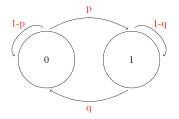
\includegraphics[width=0.3\linewidth]{figuras/cmmaq} \end{center}

Ou seja,

\(P(0,1) = P(X_{n+1}=1|X_n=0) =p\)

\(P(1,0) = P(X_{n+1}=0|X_n=1) =q\)

\(P(0,0) = P(X_{n+1} =0|X_n=0)=1-p\)

\(P(1,1) = P(X_{n+1}=1|X_n=1)=1-q\)

\subsection{Distribuição do Processo}\label{distribuicao-do-processo}

Antes de fazermos a distribuição do processo lembramos que:

\BeginKnitrBlock{theorem}[Probabilidade Total]
\protect\hypertarget{thm:unnamed-chunk-23}{}{\label{thm:unnamed-chunk-23}
\iffalse (Probabilidade Total) \fi{}
}\[X,Y = P(X=x) = \sum_y P(X=x,Y=y)\]
\EndKnitrBlock{theorem}

PROBABILIDADE CONDICIONAL

\[P(X=x,Y=y) = P(Y=y|X=x)P(X=x)\]

\begin{equation}
\begin{split}
P(X_{n+1}=0) &= P(X_{n+1}=0,X_{n}=0) + P(X_{n+1}=0,X_n=1) \\
&= P(X_{n+1}=0|X_n = 0)P(X_n=0) + P(X_{n+1}=0|X_n = 1)P(X_n=1)\\
&= (1-p)P(X_n=0) + qP(X_n=1) \text{  // observe que }P(X_n=1)=1 -
P(X_n=0)\\
&= (1-p)P(X_n=0)+ q(1-P(X_n=0))\\
&= (1-p-q)P(X_n=0) + q
\end{split}
\end{equation}

seja n = 0

\begin{equation}
\begin{split}
P(X_1=0) &= (1-p-q)\overbrace{P(X_0=0)}^{\prod_0(0)} + q\\
&=(1-p-q)\prod_0(0) + q
\end{split}
\end{equation}

Seja n = 1

\begin{equation}
\begin{split}
P(X_2=0)&=(1-p-q)P(X_1=0) + q \text{ // utilizando o resultado
anterior}\\
&= (1-p-q)[(1-p-q)\prod_0(0) + q] + q\\
&= (1-p-q)^2 \prod_0(0) + (1-p-q)q + q\\
&= (1-p-q)^2\prod_0(0) + q(1-p-q + 1)
\end{split}
\end{equation}

Seja n = 2

\begin{equation}
\begin{split}
P(X_3=0)&=(1-p-q)P(X_2=0) + q \text{ // utilizando o resultado
anterior}\\
&= (1-p-q)[(1-p-q)^2\prod_0(0) + (1-p-q)q + q] + q\\
&= (1-p-q)^3 \prod_0(0) + (1-p-q)q + (1-p-q)^2q + q\\
&= (1-p-q)^3 \prod_0(0) + q(1 + (1-p-q) + (1-p-q)^2)
\end{split}
\end{equation}

Forma geral

\[P(X_n=0)=(1-p-q)^2\prod_0(0) + q \sum_{j=0}^{n-1}(1-p-q)^j\]

Vamos supor que p + q \textgreater{} 0 logo:

PROGRESSÃO GEOMETRICA

\[\sum_{j=0}^{n-1} r^j = \frac{1-r^m}{1-r}\]

No nosso caso:

\[\sum_{j=0}^{n-1} (1-p-q)^j = \frac{1-(1-p-q)^n}{p+q}\]

Finalmente

\[P(X_n=0)= \frac{q}{p+q} + (1-p-q)^n[\prod_0(0) - \frac{q}{p+q}]\]

\[P(X_n=1)= \frac{p}{p+q} + (1-p-q)^n[\prod_0(1) - \frac{p}{p+q}]\]

OBS:

Distribuição limite

\[\underset{n \to \infty}{lim} P(X_n=0) = \frac{q}{p+q}\]

\[\underset{n \to \infty}{lim} P(X_n=1) = \frac{p}{p+q}\]

\subsection{Forma matricial}\label{forma-matricial}

Temos conhecido as probabilidades:

\[P(X_{n+1} = 1| X_n = 0) = P(0,1) = p\]

\[P(X_{n+1}|X_n=1) = P(1,0) = q\]

Podemos colocar essas probabilidades na forma de uma matriz.

\begin{equation}

P = \begin{bmatrix}
P(0,0) & P(0,1) \\
P(1,0) & P(1,1)
\end{bmatrix} =
\begin{bmatrix}
1-p & p \\
q & 1-q
\end{bmatrix}

\end{equation}

A matriz P será chamada de matriz de transição de \textbf{um passo}.

Carácteristicas da Matriz:

\begin{itemize}
\item
  Matriz quadrada
\item
  Matriz estocástica
\item
  significa que a soma das linhas é igual a 1.
\end{itemize}

\subsection{Espaços de estados}\label{espacos-de-estados}

Seja \{\(X_n\), n \(\geq\) 0\} uma CM com \(\overbrace{\text{espaços de
estados}}^{\text{o 'passo'}}\) S definimos a função de transição a 1
passo como P(x,y)=P(\(X_{n+1}\)=y\textbar{}\(X_n\)=n).

Notar que P(x,y) é uma distribuição de probabilidade pois
\(P(x,y) \geq 0\) e
\(\underbrace{\sum_{y \in S} P(x,y) = 1}_{\text{soma das linhas}}, x \in S\)

A função \(\prod_0(x)\), x \(\in\) S, definido por
\(\prod_0(x)=P(X_0=x), x \in S\) é chamada de \textbf{distribuição
inicial} do CM.

Também, \(\prod_0(x) \geq 0\) e
\(\sum_{x \in S}\underbrace{\prod_0(x_i)}_{\text{instante inicial}}=1\).

Pode ser provado que a distribuição da cadeia em qualquer instante fica
completamente determinado pelo conhecimento das probabilidades de
transição e pela distribuição normal.

\BeginKnitrBlock{example}
\protect\hypertarget{exm:unnamed-chunk-24}{}{\label{exm:unnamed-chunk-24} }

\begin{equation}
\begin{split}

P(X_0=x_0,X_1=x_1) &= \overbrace{P(X_1=x_1 | X_0 = x_0)}^{P(x_0,x_1)} \overbrace{P(X_0=x_0)}^{\prod_0(x)}\\
&= P(x_0,x_1) \prod_0(x)
\end{split}
\end{equation}

Da mesma forma \(P(X_0=x_0,X_1=x_1,X_2=x_2)\)

\begin{equation}
\begin{split}
P(\overbrace{X_0=x_0,X_1=x_1}^{A},\overbrace{X_2=x_2}^{B}) &= P(X_2 =
x_2 | X_0 = x_0, X_1 = x_1) P(X_1=x_1|X_0=x_0) P(X_0=x_0)\\
&= P(X_2 = x_2, X_1 = x_1) P(x_0,x_1)\prod_0(x_0) \text{\\ corta-se }
X_0 \text{ por que é uma CM}\\
&= \prod_0(x_0) P(x_0,x_1) P(x_1,x_2)
\end{split}
\end{equation}

\section{Fórmula geral}\label{formula-geral}

Em geral, a distribuição da cadeia vai ser:

\[P(X_0 = x_0, X_1 = x_1,...,X_n=x_n) = \prod_0(x_0) P(x_0,x_1)
P(x_1,x_2) ... P(x_{n-1},x_{n})\]
\EndKnitrBlock{example}

\BeginKnitrBlock{example}
\protect\hypertarget{exm:Exemploux20daux20muxe1quina}{}{(\#exm:Exemplo
da máquina) } No exemplo da máquina que queremos calcular a
probabilidade da máquina estar funcionando hoje e estar funcionando
ainda depois de amanhã. Ou seja, precisamos calcular:

\begin{equation}
\begin{split}
P(X_{n+2} = 1| X_n=1) &= P(1,0) \* P(0,1) + P(1,1) \* P(1,1)\\
&= qp + (1-q)(1-q)\\
&=pq + (1-q)^2
\end{split}
\end{equation}

As probabilidades de transição a n-passos podem ser facilmente obtidas
pela matriz \(P^n\) sendo:

\[P^n = p*p*...*p\]

No exemplo:

\begin{equation}
P^2 = \begin{bmatrix}
1-p & p \\
q & 1-q
\end{bmatrix}

\begin{bmatrix}
1-p & p \\
q & 1-q
\end{bmatrix}
=

\begin{bmatrix}
(1-p)^2 +pq &  (1-p)p + (1-q)p \\
q(1-p) + q(1-q) & pq + (1-q)^2
\end{bmatrix}
\end{equation}

Em resumo, a função de transição a n-passos \(P^n(x,y)\) é definida por:

\[P^n(x,y)= \sum_{y_1} ... \sum_{y_{n-1}} P(x_1,y_1) P(y_1,y_2)
... P(y_{n-1},y_n)\]
\EndKnitrBlock{example}\\[2\baselineskip]\BeginKnitrBlock{proposition}

\protect\hypertarget{prp:Fuxf3rmulaux20deux20CHAPMAN-KOLMOGOROV}{}{(\#prp:Fórmula
de CHAPMAN-KOLMOGOROV) }\[P^{n+m}(x,y) = \sum_z P^n(x,z) P^m(z,y)\]

Para uma CM com espaços de estados finitos a matriz \(P^n\) será uma
matriz finita.

Notar que a:

\begin{equation}
\begin{split}
P(X_n=y) &= \sum_{x \in S} P(X_0=x,X_n=y)\\
&= \sum_{x \in S} \overbrace{P(X_n=y|X_0=x)}^{P^n}
\overbrace{P(X_0=x_0)}^{\prod_0(x)}\\
&= \sum_{x \in S} \prod_0(x) P^n(x,y).
\end{split}
\end{equation}

Matricialmente, \(\prod_n=\prod_0P^n\)

sendo que \(\prod_n\) é a distribuição de \(X_n\)
\EndKnitrBlock{proposition}

\section{Extensões da Cadeia de
Markov}\label{extensoes-da-cadeia-de-markov}

\subsection{Construção do Modelo}\label{construcao-do-modelo}

Ideia geral de como começar o processo de modelagem dos dados.

Primeiro defina as hipóteses do processo, suposições para faciliar o
tratamento matemático.

Segundo, defina quem é o \(X_n\) se perguntando ``O que estou tentando
modelar?''.

Terceiro, defina o S e T, o espaço de estados e espaço de parâmetros.

\subsection{Passeio aleátorio}\label{passeio-aleatorio}

Sejam \(\zeta_1, \zeta_2, ...\) VA independentes, de valor inteiro com
função de probabilidade f. Seja \(X_n\) a variável aleátoria definida
por:

\[X_n = X_0 + \zeta_1 + \zeta_2 + ... + \zeta_n\]

sendo \(X_0\) o valor inicial.

A sequência \{\(X_n\), n \(\geq\) 0\} é chamado de passeio aleátorio.
Pode ser provado que é uma CM com espaço de estados inteiro e função de
transição dada por :

\[P(X,Y) = f(y-x)\]

\BeginKnitrBlock{example}
\protect\hypertarget{exm:unnamed-chunk-25}{}{\label{exm:unnamed-chunk-25} }
Suponha que uma particula se movimenta de acordo com essa cadeia.
Consideremos o caso especial f(1) = p e f(-1) = q e f(0) = r, com p + q
+ r = 1.

A função de transição será:

\begin{equation}
P(x,y) = \left\{\begin{matrix}
p & y = x + 1 \\
q & y = x - 1\\
r & y = x
\end{matrix}\right.

\end{equation}

Essa cadeia particular é chamada de passeio aleátorio simples, ou
passeio do bêbado.
\EndKnitrBlock{example}

\begin{center}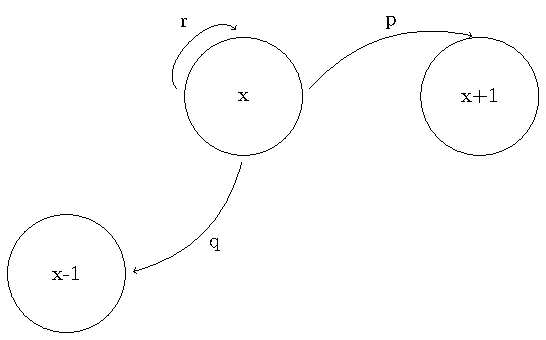
\includegraphics[width=1\linewidth,height=250x]{./figuras/pe2} \end{center}

Por exemplo se S = \{0,1,2,\ldots{}\}

\begin{center}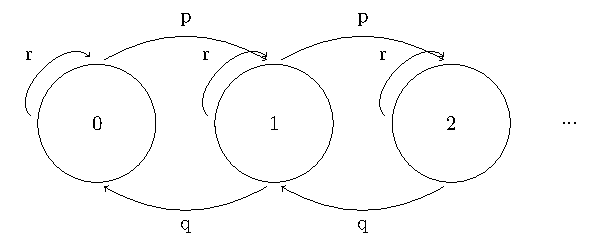
\includegraphics[width=1\linewidth,height=250px]{./figuras/pe3} \end{center}

A matriz de transição fica como segue-se:

\begin{tabular}{l|c|c|c|c|c}
\hline
  & 0 & 1 & 2 & 3 & ...\\
\hline
0 & r0 & p & 0 & 0 & \\
\hline
1 & q & r & p & 0 & \\
\hline
2 & 0 & q & r & p & \\
\hline
3 & 0 & 0 & q & r & \\
\hline
... &  &  &  &  & $\ddots$\\
\hline
\end{tabular}

\subsection{Cadeia de Ehrenfest}\label{cadeia-de-ehrenfest}

Paul Ehrenfest nasceu em 18/01/1880 e morreu no dia 25/07/1993. Ele foi
um físico teórico alemão que teve suas maiores contribuições feitas no
campo da estatística mecânica, mecânica quântica , incluindo o a teoria
de fase de transição, e o teorema de Ehrenfest.
\href{https://en.wikipedia.org/wiki/Paul_Ehrenfest}{Referência}

O seguinte modelo pode ser utilizado para intercambio de moleculas de um
gás entre corpos isolados.

Suponha que temos duas caixas numeradas I e II e \textbf{d} bolas,
também numeradas de 1 a \textbf{b}. Inicialmente algumas bolas são
colocadas na caixa I e as restantes na caixa II. Um inteiro é
selecionado aleatoriamente do conjunto \{1,2,\ldots{},d\} e a bola
correspondente a esse número é trocada de caixa. Repete-se esse processo
indefinidamente. Com seleções independentes entre os ensaios. Seja
\(X_n\): número de bolas na caixa I após a n-esimo ensaio.

Pode ser provado que \{\(X_n\), n \(\geq\) 0\} é uma cadeia de markov
sobre S = \{0,1,2,3,\ldots{},d\} (T=\{0,1,2,3,\ldots{})

Precisamos encontrar a função de transição P(x,y) \(\forall\) (x,y)
\(\epsilon\) S, para tal vamos supor que em determinado instante temos x
bolas na caixa I. Vemos então que as únicas transições possíveis são:

\begin{equation}
x \rightarrow x-1 \\
x \rightarrow x + 1
\end{equation}

\begin{equation}
P(x,x-1) = \frac{x}{d}\\
P(x,x+1) = \frac{d-x}{d} = 1 - \frac{x}{d}
\end{equation}

Logo a função de transição é:

\begin{equation}
P(x,y)\left\{\begin{matrix}
\frac{x}{d} &; y = x - 1 \\
\frac{d-x}{d} &; y = x+1\\
0 &; cc
\end{matrix}\right.
\end{equation}

Matriz de transição.

\begin{tabular}{l|c|c|c|c|c|c}
\hline
  & 0 & 1 & 2 & 3 & ... & d\\
\hline
0 & 0 & 1 & 0 & 0 & ... & 0\\
\hline
1 & $\frac{1}{d}$ & 0 & $1 - \frac{1}{d}$ & 0 & ... & 0\\
\hline
2 & 0 & $\frac{2}{d}$ & 0 & $1 - \frac{2}{d}$ & ... & 0\\
\hline
3 & 0 & 0 & 0 & 0 & ... & 0\\
\hline
... & ... & ... & ... & ... & ... & 0\\
\hline
d & 0 & 0 & 0 & 0 & 1 & 0\\
\hline
\end{tabular}

\subsection{Ruína do jogador}\label{ruina-do-jogador}

Suponha que um jogador faz apostas de um dolar por vez, sendo que sua
probabilidade de ganhar é \texttt{p}. Seja \(X_0\) o capital inicial do
jogador. Suponha ainda que não existe ``emprestimo'' da banca, ou seja,
o jogador deixa de jogar se o seu capital atingir 0, nessa caso diremos
que o jogador está arruinado.

Seja \(X_n\) : capital do jogador no instante n:

\[{X_n, n \geq 0} \text{uma CM. sobre {0, 1, 2, ...}}\]

\begin{equation}
P(x,y )\left\{\begin{matrix}
 1-p &, y = x -1\\
p  &, y = x + 1\\
0 &,  cc
\end{matrix}\right.
\end{equation}

\BeginKnitrBlock{definition}
\protect\hypertarget{def:unnamed-chunk-30}{}{\label{def:unnamed-chunk-30}
}Um estado a \(\epsilon\) S de uma cadeia de Markov será chamado de
absorvente se P(a,a) = 1. (ou equivalentemente, P(a,x)=0,
\(\forall x \neq a\))

Vamos supor que o jogo seja definido se o ganho do jogador atingir
\texttt{d} dolares ele deve abandonar o jogo. Nesse caso, S = \{
0,1,2,\ldots{},d\}

Essa cadeia é chamada ``com barreiras absorventes''
\EndKnitrBlock{definition}

\subsection{\texorpdfstring{Cadeia de Nascimento e Morte \textbf{(C
N-M)}}{Cadeia de Nascimento e Morte (C N-M)}}\label{cadeia-de-nascimento-e-morte-c-n-m}

Considere uma CM sobre S = \{0,1,2,\ldots{}\} ou sobre S =
\{0,1,2,\ldots{}d\} e suponha a seguinte função de transição.

\begin{equation}
P(x,y)\left\{\begin{matrix}
q_x &, y = x -1\\
r_x &, y = x \\
p_x &, y = x + 1 \\
0 & cc
\end{matrix}\right.
\end{equation}

Sendo \(p_x, q_x, r_x\) inteiros não negativos tal que
\(p_x + q_x + r_x = 1\)

A matriz de transição fica:

\begin{tabular}{l|l|l|l|l|l|l}
\hline
  & 0 & 1 & 2 & 3 & ... & d\\
\hline
0 & $r_0$ & $p_0$ & 0 & 0 & ... & 0\\
\hline
1 & $q_1$ & $r_1$ & $p_1$ & 0 & ... & 0\\
\hline
2 & 0 & $q_2$ & $r_2$ & $p_2$ & ... & 0\\
\hline
... & ... & ... & ... & ... & ... & 0\\
\hline
d & 0 & 0 & 0 & 0 & $q_d$ & $r_d$\\
\hline
\end{tabular}

NOTAR: que o passeio aleátorio, a cadeia de Ehrenfest e a ruína do
jogador são casos particulares de C N-M.

\subsection{Cadeia de Fila}\label{cadeia-de-fila}

Considere um sistema de serviço em que os clientes chegam e devem
esperar por atendimento formando uma fila.

Suponha que se há clientes esperando serviço no inicio de qualquer
período de tempo, exatamente um cliente será atendido nesse período (não
existe atendimentos simultaneos). E que se não há clientes esperando
então ninguém será atendido nesse período.

Seja \(\zeta_n\) o número de novos clientes que chegam durante o período
(n-esimo).

Vamos supor que as variáveis aleátorias \(\zeta_1, \zeta_2,... \zeta_n\)
são independentes e identicamente distribuidas segundo uma função de
probabilidade f.

Seja \(X_0\) o número inicial de clientes e \(X_n\) o número de clientes
no sistema até o final do n-esimo período.

Se \(X_n\) = 0, então \(X_n + 1 = \zeta_{n + 1}\)

Se \(X_n \geq 1\), então \(X_n + 1 = X_n + \zeta{n+1} - 1\)

Então \{\(X_n, n \geq\)\} é uma CM sobre \{0,1,2,\ldots{}\} com função
de transição

P(x,y) = f(y-x+1) \(x \geq 1\)

P(0,y) = f(y)

\subsection{Cadeia de ramificação}\label{cadeia-de-ramificacao}

Considere objetos tais como particulas de algum tipo ou bacterias que
podem gerar novos elementos do mesmo tipo.

O conjunto inicial de objetos será chamado ``geração zero''. Os
elementos gerados durante o n-esimo tempo serão dito pertencer a
(n+1)-esima geração.

Seja \(X_n\) o nº de objetos no n-esima geração, então temos, por
exemplo a seguinte situação.

\begin{center}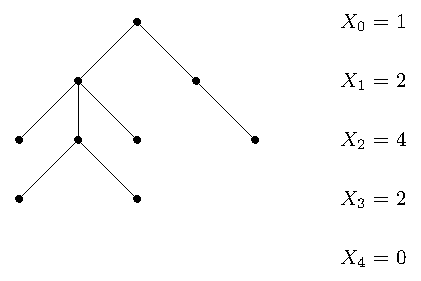
\includegraphics{./figuras/pe4} \end{center}

Para modelar essa situação como uma CM vamos supor que cada particula
gera \(\zeta\) novas particulas na próxima geração, sendo \(\zeta\) uma
VA de valor inteiro não negativo, tendo a função de probabilidade f. Sob
essa hipótese \{\(X_n\), n \(\geq\) 0\} será uma CM cujo o espaço de
estados é S = \{0,1,2,3,\ldots{}\}.

Notar que 0 é um estado absorvente.

Se a cadeia atingir o estado 0, diremos que ela foi extinta, e um
problema muito interessante é determinar a probabilidade de extinção da
cadeia.

Para x \(\geq\) 1 a função de transição será:

P(x,y) = P(\(\zeta_1 + \zeta_2 + ... + \zeta_x = y)\)

com os \(\zeta_i\)'s sendo iid com f.d.p e

P(1,y) = f(y), \(y \geq 0\)

\BeginKnitrBlock{definition}
\protect\hypertarget{def:unnamed-chunk-33}{}{\label{def:unnamed-chunk-33}
}Seja A um subconjunto de S. Define-se o tempo de chegada (hitting time)
em A como:

\(T_A = min\{n \geq 0: X_n \epsilon A\}\), se \(X_n \epsilon A\), para
algum n \(\geq\) 0.
\EndKnitrBlock{definition}\\
\BeginKnitrBlock{definition}
\protect\hypertarget{def:unnamed-chunk-34}{}{\label{def:unnamed-chunk-34}
}\(T_A\) = \(\infty\) se \(X_n\) \(\not{\epsilon}\) A, \(\forall\) n
\textgreater{} 0.
\EndKnitrBlock{definition}\\
Ou seja, \(T_A\) é o primeiro indice de \(X_n\) em que a cadeia entra no
conjunto A pela primeira vez.

\begin{description}
\tightlist
\item[NOTAÇÃO]
Quando A = \{y\}, em lugar de escrever \(T_{{y}}\) vamos apenas escrever
\(T_y\).
\item[NOTAÇÃO]
Denotaremos por \(P_x\)(A) a probabilidade de A ocorrer quando a CM
começou no estado x. Por exemplo, \(P_x\)(\(X_5 = 2\)) ou \(P_0(T_y=3)\)
``A probabilidade,saindo de zero a cadeia, atingir o estado y, pelo
menos uma vez.''
\end{description}

\section{Estados Transientes e
Recorrentes}\label{estados-transientes-e-recorrentes}

Seja \{\(X_n\), n \(\geq\) 0\} uma CM sobre S com função de transição
p(x,y). Definida como:

\[\rho_{xy} = \rho(T_y \leq \infty)\]

I.E, a probabilidade de saindo de x, atingir o estado y em um tempo
finito.

Em particular, \(\rho_{yy}\) denota a probabilidade de sair de y e
retornar para y (alguma vez) -\textgreater{} tempo finito.

\BeginKnitrBlock{definition}
\protect\hypertarget{def:unnamed-chunk-35}{}{\label{def:unnamed-chunk-35}
}Diremos que um estado y é \textbf{transiente} se \(\rho \leq 1\).
\EndKnitrBlock{definition}

Isto quer dizer que, se y for recorrente, então, com probabilidade 1, a
cadeia retornará alguma vez em y.

Se y for transiente, existe uma probabilidade positiva (de valor 1 -
\(\rho_{yy}\)) de sair de y e não retornar.

Seja N(y) o número de vezesque a cadeia \textbf{VISITA} o estado y
(\(n \geq 1\)).

Então, \(P_x\) (N(y) \(\geq\) 1 ) = \(P_x\) (\(T_y \leq \infty\)) =
\(\rho_{xy}\).

Denotaremos por EX(.) a esperança de alguma VA, com a cadeia partindo em
x.

\BeginKnitrBlock{theorem}
\protect\hypertarget{thm:unnamed-chunk-36}{}{\label{thm:unnamed-chunk-36}
}i) Se y é transiente, então \(F_x\)(N(y) \textless{} \(\infty\)) = 1 e
E(N(y)) = \(\frac{\rho_{xy}}{1-\rho_{yy}}\), x \(\epsilon\) S ii) Se y é
recorrente, então \(P_x(N(y) = \infty)\) = 1 e \(E_x(N(y))\)
=\(\infty\).
\EndKnitrBlock{theorem}

Isto significa que estados transientes são apenas estados de
``passagem'' ou transitórios, enquanto que estados recorrentes são
estados permanentes ou definitivos. Isso produz uma partição do espaço
de estados.

\[S = S_T \cup S_R, (S_T \cap S_R = \varnothing)\]

\BeginKnitrBlock{definition}
\protect\hypertarget{def:unnamed-chunk-37}{}{\label{def:unnamed-chunk-37}
}Sejam x e y dois estados de S. Diremos que x atinge y se \(\rho_{xy}\)
\textgreater{} 0.
\EndKnitrBlock{definition}\\
NOTAÇÃO : (independente do número de passos): x \(\rightarrow\) y.
``Saindo de x em n passos chego em y''

\BeginKnitrBlock{definition}
\protect\hypertarget{def:unnamed-chunk-38}{}{\label{def:unnamed-chunk-38}
}Diremos que dois estados quaisquer estão comunicados se x
\(\rightarrow\) y e y \(\rightarrow\) x.
\EndKnitrBlock{definition}\\
\BeginKnitrBlock{theorem}
\protect\hypertarget{thm:unnamed-chunk-39}{}{\label{thm:unnamed-chunk-39}
}Seja X um estado recorrente. Suponha que x \(\leftrightarrow\) y. Então
y será também recorrente. Aqui \(\rho_{xy}\) = \(\rho_{yx}\) = 1. (Isso
significa que estados se comunicam somente com estados de mesma
natureza)
\EndKnitrBlock{theorem}\\
\BeginKnitrBlock{definition}
\protect\hypertarget{def:unnamed-chunk-40}{}{\label{def:unnamed-chunk-40}
}1) Um conjunto C estados é chamado \textbf{fechado} se \(\rho_{xy}\) =
0, x \(\leq\) c, y \(\notin\) c. 2) Um conjunto c é chamado irredutivel
se x \(\leftrightarrow\) y, \(\forall\) x,y \(in\) c. (Ou seja, todos os
estados de c estão comunicados)
\EndKnitrBlock{definition}\\
\BeginKnitrBlock{theorem}
\protect\hypertarget{thm:unnamed-chunk-41}{}{\label{thm:unnamed-chunk-41}
}Seja C um conjunto finito irredutivel e fechado de estados. Então,
todos os estados em C serão recorrentes.
\EndKnitrBlock{theorem}\\
C é o conjunto de estados. FINITO, FECHADO e IRREDUTÍVEL.\\
\BeginKnitrBlock{example}
\protect\hypertarget{exm:unnamed-chunk-42}{}{\label{exm:unnamed-chunk-42} }
Considere uma cadeia de markov com matrix de transição MT
\EndKnitrBlock{example}

% Please add the following required packages to your document preamble:
% \usepackage[table,xcdraw]{xcolor}
% If you use beamer only pass "xcolor=table" option, i.e. \documentclass[xcolor=table]{beamer}
\begin{table}[h]
\centering
\caption{}
\begin{tabular}{|c|c|c|c|c|c|c|}
\hline
0 & \cellcolor[HTML]{FE0000}1 & 2   & 3    & 4                                         & 5                                         &                              \\ \hline
0 & 1                         & 0   & 0    & 0                                         & 0                                         & 0                            \\ \hline
1 & 0.25                      & 0.5 & 0.25 & 0                                         & 0                                         & 0                            \\ \hline
2 & 0                         & 0.2 & 0.4  & 0.2                                       & 0                                         & 0.2                          \\ \hline
3 & 0                         & 0   & 0    & \cellcolor[HTML]{FE0000}0.166666666666667 & \cellcolor[HTML]{FE0000}0.333333333333333 & \cellcolor[HTML]{FE0000}0.5  \\ \hline
4 & 0                         & 0   & 0    & \cellcolor[HTML]{FE0000}0.5               & \cellcolor[HTML]{FE0000}0                 & \cellcolor[HTML]{FE0000}0.5  \\ \hline
5 & 0                         & 0   & 0    & \cellcolor[HTML]{FE0000}0.25              & \cellcolor[HTML]{FE0000}0                 & \cellcolor[HTML]{FE0000}0.75 \\ \hline
\end{tabular}
\end{table}

S = \{0,1,2,3,4,5\}

Como os conjuntos \(C_1\) = \{0\} e \(C_2\) = \{3,4,5\} são finitos,
fechados e irredutiveis, então eles são conjuntos de estados
recorrentes.

Assim, \(S_R\) = \{0\} \(\cup\) \{3,4,5\} e \(S_T\) \{1,2\}

Notar que 0 é um estado absorvente, logo recorrente. 3,4 e 5 são estados
recorrentes. ``` \#\# Probabilidade de absorção

Seja C um conjunto de estados recorrentes (fechado e irredutivel) e seja
\(\rho_c\)(x) = \(P_x\) (\(T_c\) \textless{} \(\infty\)). Dado que a
cadeia permanecerá definitivamente em C, se os estados de C forem
atingidos, diremos que a cadeia foi absorvida em C e chamaremos a
\(\rho_c\)(x) de probabilidade de absorção de C, saindo do estado x.

Notar que, trivialmente

\(\rho_c(x) = 1, x \in C\)

\(\rho_c(x) =0, x \notin C\)

Vamos calcular \(\rho(x)\), x \(\in\) \(S_T\).

\BeginKnitrBlock{theorem}
\protect\hypertarget{thm:unnamed-chunk-45}{}{\label{thm:unnamed-chunk-45}
}Seja C um conjunto finito, fechado e irredutivel de estados. Então:

\[\rho_c(x) = \sum_{y \in C}P(x,y) + \sum_{y \in S_T} P(x,y)P_C(y), x
\in S_T\]
\EndKnitrBlock{theorem}

Consideramos \(C_1\) = \{0\}, x = 1 ou 2 (\(S_T = (1,2)\))

x = 1

\begin{equation}
\begin{split}
\rho_{{0}}(1) &= \sum_{y \in {0}}P(1,y) + \sum_{y \in
{1,2}}P(1,y)\rho_{{0}}(y), x \in S_T\\
\rho_{{0}}(1) &= P(1,0) + [P(1,1) \rho_{{0}}(1) + P(1,2) \rho_{{0}}(2)]\\
\rho_{{0}}(1) &= \frac{1}{4} + [\frac{1}{2} \rho_{{0}}(1) + \frac{1}{4}
\rho_{{0}}(2)]\\
\frac{1}{2} \rho_{{0}}(1) - \frac{1}{4}\rho_{{0}}(2) = \frac{1}{4} \text{ (1)
Primeira equação}
\end{split}
\end{equation}

x = 2

\begin{equation}
\begin{split}
\rho_{{0}}(2) &= \sum_{y \in {0}} P(2,y) + \sum_{y \in
{1,2}}P(2,y)\rho_{{0}}(y)\\
\rho_{{0}}(2) &= 0 + [P(2,1)\rho_{{0}}(1) + P(2,2)\rho_{{0}}(2)]\\
\frac{1}{5}\rho_{{0}}(1) - \frac{3}{5} \rho_{{0}}(2) = 0 \text{ (2)
Segunda equação}
\end{split}
\end{equation}

De (2):

\[\frac{1}{5}\rho_{{0}}(1) = \frac{3}{5}\rho_{{0}}(2) =>
\frac{1}{3}\rho_{{0}}(1)\]

De (1):

\[\frac{1}{2}\rho_{{0}}(1) - \frac{1}{4} \frac{1}{3}\rho_{{0}}(1) =
\frac{1}{4}\]

Logo:

\begin{equation}
\frac{6 \rho_{{0}}(1) - \rho_{{0}}(1)}{12} = \frac{1}{4}\\
5 \rho_{{0}}(1) = 3\\
\rho_{{0}}(1) = \frac{3}{5}
\end{equation}

Em (2):

\begin{equation}
\frac{1}{2} \frac{3}{5} - \frac{1}{4} \rho_{{0}}(2)= \frac{1}{4}\\
\rho_{{0}}(2) = \frac{1}{5}
\end{equation}

Como a cadeia só pode ser absorvente em \(C_1\) ou \(C_2\), essas
probabilidade são complementares logo:

\[\rho_{{3,4,5}}(1) = 1 - \rho_{{0}}(1) = \frac{2}{5}\]

e

\[\rho_{{3,4,5}}(2) = \frac{4}{5}\]

\subsection{Martingales}\label{martingales}

Considere uma CM sobre \{0,1,2,\ldots{},d\} com função de transição
\(\rho\) satisfazendo:

\[\sum_{y=0}^d yP(x,y) = x, x=0,...,d\]

então, E{[}\(X_{n+1}|X_0 = x_0,...,X_{n-1}=x_{n-1},X_n=x_n\){]}=x (i.e,
o valor esperado de \(X_{n+1}\) dado o passado e o presente do processo,
depende somente do valor presente.)

\BeginKnitrBlock{definition}
\protect\hypertarget{def:unnamed-chunk-46}{}{\label{def:unnamed-chunk-46}
}Uma sequência de VA'S satisfazendo a propriedade acima será chamado de
\textbf{MARTINGALES}.
\EndKnitrBlock{definition}

OBS: Na verdade um martingale não é necessariamente uma CM, mas é um
elemento importante na teoria de jogos.

\subsection{Cadeias N-M}\label{cadeias-n-m}

Quando uma CM é irredutivel, ou seja, todos seus estado são da mesma
natureza. ``Todos são transientes ou todos são recorrentes''.

Quando S é finito e a CM é irredutivel.

Todos os estados serão recorrentes. Nesse caso diremos que a cadeia é
recorrente.

Analisar os estados quando S não é finito é um problema extremamente
complexo e a natureza dos estados denpederá da existencia de algumas
estruturas probabilisticas sobre a cadeia. O caso particular das cadeias
de nascimento e morte é um dos casos em que consegue-se um criterio de
classificação de estados

\BeginKnitrBlock{definition}
\protect\hypertarget{def:unnamed-chunk-47}{}{\label{def:unnamed-chunk-47}
}Seja \{\(X_n, n \geq 0\)\} uma C-N-M com função de probabilidade.

\[
P(x,y) =\left\{\begin{matrix}
  q_x &, y = x-1\\
  r_x &, y = x \\
  p_x &, y = x +1
\end{matrix}\right.
\]
\EndKnitrBlock{definition}

sendo \(q_x + p_x + r_x\) = 1, \(\forall\) x \(\in\) S.

\[P_x(T_a < T_b) = \frac{\sum_{y=x}^{b-1} \gamma_y}{\sum_{y=a}^{b-1}}\]

sendo que:

\[\gamma_y = \frac{q_1q_2...q_y}{p_1p_2...p_y}\]

a \textless{} x \textless{} b

Ainda,

\begin{equation}
\begin{split}
P_x(T_a < T_b) &= 1 - P(T_a < T_b)\\
&= \frac{\sum_{y=a}^{x-1} \gamma_y}{\sum_{y=a}^{b-1}}
\end{split}
\end{equation}

Notar que \(P_x(T_a < T_b)\) indica a probabilidade de saindo de x
atingir o estado A antes de que o estado B.

\BeginKnitrBlock{example}
\protect\hypertarget{exm:unnamed-chunk-48}{}{\label{exm:unnamed-chunk-48} }
Um jogador faz aposstas de um dolar por vez com probabilidade
\(\frac{9}{19}\) de ganhar e \(\frac{10}{19}\) de perder. Supoha que o
jogador deixa de jogar quando está arruinado ou quando o seu lucro for
de 25 dolares. Suponha que ele inicia o jogo com capital de 10 dolares.

\subsubsection{a.}\label{a.}

Encontrar a probabilidade do jogador se retirar ganhando

Temos que \(\gamma_y\):

\[\gamma_y =
\frac{(\frac{10}{19})(\frac{10}{19})...(\frac{10}{19})}{(\frac{9}{19})(\frac{9}{19})...(\frac{9}{19})}
= \frac{(\frac{10}{19})^y}{(\frac{9}{19})^y} = (\frac{10}{9})^y\]

Logo:

\begin{equation}
\begin{split}
P_{10}(T_{35}<T_0) &= \frac{\sum_{y=0}^9
(\frac{10}{9})^y}{\sum_{y=0}^{34} (\frac{10}{9})^y}\\
&= \frac{\frac{1 - (\frac{10}{9})^{10}}{1 - \frac{10}{9}}}{\frac{1 -
(\frac{10}{9})^{35}}{1 - \frac{10}{9}}}\\
&= \frac{1 - (\frac{10}{9})^{10}}{1 - (\frac{10}{9})^{35}}= 0.047
\end{split}
\end{equation}

\subsubsection{b.}\label{b.}

Encontrar a perda esperada

\begin{equation}
L = \left\{\begin{matrix}
10 &, \text{ se atingir 0} \\
-25 &, \text{ se atingir 35}
\end{matrix}\right.
\end{equation}

\begin{equation}
\begin{split}
E(L) &= 10 P(atingir 0) - 25 P(atingir35)\\
&= 10(1x 0.047) - 25(0.047)\\
&= 10 - 35x0.047
\end{split}
\end{equation}
\EndKnitrBlock{example}\\
\BeginKnitrBlock{theorem}
\protect\hypertarget{thm:unnamed-chunk-49}{}{\label{thm:unnamed-chunk-49}
}Seja \{\(X_n, n \geq 0\)\} uma C-N-M irredutivel sobre S
=\{0,1,2,\ldots{}\}. Então, a cadeia será recorrente se:

\[\sum_{x=1}^{\infty} \gamma_x = \infty\]

caso contrario a cadeia sera transiente
\EndKnitrBlock{theorem}

\section{Distribuição estacionária de uma
CM}\label{distribuicao-estacionaria-de-uma-cm}

\BeginKnitrBlock{example}
\protect\hypertarget{exm:unnamed-chunk-50}{}{\label{exm:unnamed-chunk-50}
}Seja \{\(X_n\), n \(\geq\) 0\} uma CM com dois estados tais que:

\begin{equation}
P = \begin{bmatrix}
1/3 & 2/3 \\
1/2 & 1/2
\end{bmatrix}
\end{equation}

Temos que \(P^2\) é:

\begin{equation}
P^2 = \begin{bmatrix}
4/9 & 5/9 \\
5/12 & 7/12
\end{bmatrix}
\end{equation}

\(P^4\)

\begin{equation}
P^4 = \begin{bmatrix}
139/324 & 185/324 \\
185/432 & 247/432
\end{bmatrix}
\end{equation}
\EndKnitrBlock{example}

Intuimos que a matriz \(P^n\) \(\approx\) \(P^8\), n \textgreater{} 8.
Isto mostra que para n suficientemente grande a distribuição da cadeia
(prob de transição) tende a estabilizar em determinados valores para
todos os estados, ou seja, as linhas da matriz \(P^n\) tendem a se
igualar.

\subsection{Distribuição Estacionária de uma
CM.}\label{distribuicao-estacionaria-de-uma-cm.}

Uma pergunta interessante é saber o que acontece com a matriz \(P^n\),
para n suficientemente grande. isso tem a ver com a chamada
\textbf{distribuição estacionária}, ou de equilibrio.

\BeginKnitrBlock{definition}
\protect\hypertarget{def:unnamed-chunk-51}{}{\label{def:unnamed-chunk-51}
}Seja \{\(X_n n \geq 0\)\} uma CM sobre S com função de transição P.
Diremos que uma distribuição de probabilidade \{\(\Pi(x)\), x \(\in\)
S\} é uma distribuição estacionária se:
\[ \sum_x \Pi(x) P(x,y) = \Pi(y), y \in S\]
\EndKnitrBlock{definition} Matricialmente a condição para ser DE
(distribuição estacionária)

\[\Pi P = \Pi\]

sendo que \(\Pi\) é um vetor de probabilidades e P a matriz de
transição.

\BeginKnitrBlock{example}
\protect\hypertarget{exm:unnamed-chunk-52}{}{\label{exm:unnamed-chunk-52} }

Para P, consideramos \(\Pi = (\Pi(0),\Pi(1))\)

\begin{equation}
P = \begin{bmatrix}
1/3 & 1/3 \\
1/2 & 1/2
\end{bmatrix}
\end{equation}

Temos que:

\begin{equation}
(\Pi(0),\Pi(1)) \begin{bmatrix}
1/3 & 2/3 \\
1/2 & 1/2
\end{bmatrix} = (\Pi(0),\Pi(1))
\end{equation}

I. \(\frac{\Pi_0}{3} + \frac{\Pi_1}{2} = \Pi_0\)

\begin{enumerate}
\def\labelenumi{\Roman{enumi}.}
\setcounter{enumi}{1}
\item
  \(\frac{2\Pi_0}{3} + \frac{prod_1}{2} = \Pi_1\)
\item
  \(\frac{\Pi_0 + \Pi_1} = 1\)
\end{enumerate}

A III eq foi acrescentada por que sabemos que a soma das duas
probabilidades \(\Pi\) tem que resultar em 1. Assim o sistema de
equações agora tem solução.

I em III

\(\Pi_0 + \frac{4}{3} \Pi_0 = 1 => \Pi_0 = \frac{3}{7}\)

e

\(\Pi_1 = \frac{4}{7}\)
\EndKnitrBlock{example}\\
Quando temos uma cadeia com infinitos estados, não é possível resolver o
sistema \(\Pi P = \Pi\) para obter a distribuição estacionária.

No caso particular de C-N-M é possível encontrar a DE.

Considere uma cadeia de nascimento e morte sobre \{0,1,2\ldots{}\} ou
sobre \{0,1,2,3,4,\ldots{},d\}, tal que:

\begin{equation}
\begin{matrix}
p_x > 0 &, p/ 0 \leq x \leq d \\
q_x > 0 &, p/ 0 \leq x \leq d
\end{matrix}
\end{equation}

A condição de estcionariedade é: \(\sum_x \Pi(x) P(x,y)= \Pi(x,y)\)

Isto é:

y = 0

\begin{equation}
\begin{split}
\sum_x \Pi(x)P(x,0) &= \Pi(0)\\
\Pi(0)P(0,0) + \Pi(1) P(1,0) + \Pi(2) P(2,0)... &= \Pi(0)\\
\Pi(0)r_0 + q_1\Pi(1) + 0 + 0 + 0 ... &= \Pi(0)\\
q_1 \Pi(1) + \Pi(0)[r_0 -1] &= 0\\
q_1\Pi(1) - \Pi(0)p_0 &= 0\\
\Pi(1) &= \frac{p_0}{q_1} \Pi(0)
\end{split}
\end{equation}

Para qualquer y: \(\sum_x \Pi(x) P(x,y) = \Pi(y)\)

\[\Pi(y-1)P(y-1,y) + \Pi(y)P(y,y) + \Pi(y+1) P(y+1,y) = \Pi(y)\]

y = 1

\begin{equation}
\begin{split}
P_0 \Pi(0) + r_1 \Pi(1) + q_2 \Pi(2) &= \Pi(1)\\
q_2\Pi(2) &= (1 - r_1) \Pi(1) - p_0\Pi(0)\\
q_2\Pi(2) &= (p_1 + q_1) \Pi(1) - p_0\Pi(0)\\
q_2\Pi(2) &= (p_1 + q_1) \frac{p_0}{q_1} \Pi(0) - p_0\Pi(0)\\
q_2\Pi(2) &= \Pi(0)[\frac{p_1p_0}{q_1} + p_0 - p_0]\\
\Pi(2) &= \frac{p_1 p_0}{q_1 q_2} \Pi(0)
\end{split}
\end{equation}

Em geral

\[\Pi(x) = \frac{p_0 p_1 ... p_{x-1}}{q_1 q_2 ... q_x} \Pi(x)\]

Define-se

\begin{equation}
\alpha\left\{\begin{matrix}
1 &, x = 0 \\
\frac{p_0 p_1 ... p_{x-1}}{q_1 q_2 ... q_x} \Pi(x) &  x \geq 0
\end{matrix}\right.
\end{equation}

Assim, \(\Pi(x)\) = \(\alpha_x \Pi(0)\), \(x \geq 0\)

Somando em ambos os lados

\[\sum_x \Pi(x) = \sum_x \alpha_x \Pi(0)\]

\[1 = \Pi(0) \sum_x \alpha_x\]

Logo:

\[\Pi(0) = \frac{1}{\sum_{x=0}^{\infty} \alpha_x}\]

Se \(\sum_{x=0}^{\infty} \alpha_x < \infty\), então existe uma DE que
será dada por:

\[\Pi(x) = \frac{\alpha_x}{\sum_{x=0}^{\infty}\alpha_x}\]

OBS: Isto para uma C-N-M

\section{Distribuição estacionária de uma
CM}\label{distribuicao-estacionaria-de-uma-cm-1}

\subsection{Método de Decomposição
Especial}\label{metodo-de-decomposicao-especial}

Para encontrar a matriz \(P^n\) no caso de dois estados.

Seja

\begin{equation}
P = \begin{bmatrix}
1 - a & a \\
b &  1-b
\end{bmatrix}
\end{equation}

0 \textless{} a \textless{} 1, 0 \textless{} b \textless{} 1.

\(P^n\) = \(\lambda_1^n E_1 + \lambda_2^n E_2\), sendo \(\lambda_1\) e
\(\lambda_2\) os autovalores da equação caracteristica.

\[det(\lambda I-P) = 0\]

I identidade

As matrizes \(E_1\) e \(E_2\) são dadas por:

\[E_1 = \frac{1}{\lambda_1 - \lambda_2} [P - \lambda_2I]\]

\[E_2 = \frac{1}{\lambda_2 - \lambda_1} [P - \lambda_1I]\]

\subsection{DE p/ C-N-M}\label{de-p-c-n-m}

\[\pi(x)= \frac{\alpha x}{\sum_{y=0} \alpha_y}, x \geq 0\]

\begin{equation}
\alpha_x = \left\{\begin{matrix}
1 &, x =0 \\
\frac{p_0...p_{x-1}}{q_1...q_x} &, x \geq 1
\end{matrix}\right.
\end{equation}

\subsection{Cadeia de Ehrenfest
Modificada}\label{cadeia-de-ehrenfest-modificada}

Tem-se \textbf{d} bolas numeradas e duas caixas (I e II). Inicialmente
\textbf{m} bolas são distribuidas de forma aleatoria nas duas caixas.
Seleciona-se um número inteiro entre 1 e \textbf{d}, retira-se a
correspondente a esse número e logo recoloca-se numa das caixas
selecionadas aleatoriamente. O interesse é o número de bolas na caixa I.

Seja \(X_n\): o nº de bolas na caixa I, após o n-esimo sorteio. Então,
\{\(X_n\), n \(\geq\) 0\} será uma CM sobre S = \{0,1,\ldots{},d\}.

No caso de d = 3, temos que:

\(p_0\) = 1/2 \(p_1\) = 1/3 \(p_2\) = 1/6\\
\(q_1\) = 1/6 \(q_2\) = 1/3 \(q_3\) = 1/2\\

\begin{equation}
P = \begin{bmatrix}
1/2 & 1/2 & 0 & 0 \\
1/6 & 3/6 & 1/6 & 0\\
0 & 2/6 & 3/6 & 1/6\\
0 & 0 & 1/2 & 1/2
\end{bmatrix}
\end{equation}

\(\alpha_0=1\) \(\alpha_1= \frac{p_0}{p_1} = \frac{1/2}{1/6}=3\)\\
\(\alpha_2=\frac{p_0p_1}{q_1q_2}=\frac{1/2 x 1/3}{1/6 x 1/3} = 3\)\\
\(\alpha_3=\frac{p_0p_1p_2}{q_1q_2q_3}=\frac{1/2 x 1/3 x 1/6}{1/2 x 1/3 x 1/2}= \frac{3 x 1/6}{1/2}\)\\
\(\alpha_3=1\)

\(\sum_{y=0}^3 \alpha_y = \alpha_0 + \alpha_1 + \alpha_2 + \alpha_3 = 1 + 3 + 3 + 1 = 8\)

\(\pi(0) = \frac{\alpha_0}{\sum \alpha_y} = 1/8\)
\(\pi(1) = \frac{3}{\sum \alpha_y}=\frac{3}{8}\)\\
\(\pi(2)=3/8\) \(\pi(3)=1/8\)

\(\pi\) = (1/8,3/8,3/8,1/8)\$

Seja \(N_n(y)\) o número de visitas da cadeia no estado y durante os
tempos m = 1,\ldots{},n. Denotado por Gn(x,y) o valo esperado da VA.
Nn(y), quando a cadeia come em x, isto é:

\[Gn (x,y) = E_x(Nn(y))\]

Quando y é transiente, o limite Nn(y) \textless{} \(\infty\). Seja y
recorrente e consideremos my = \(E_y\)(\(T_y\)) (tempo medio de retorno
em y)

\BeginKnitrBlock{definition}
\protect\hypertarget{def:unnamed-chunk-53}{}{\label{def:unnamed-chunk-53}
}Um estado recorrente será chamado recorrente nulo se my = \(\infty\)\\
Caso contrario (ie, se my \textless{} \(\infty\)) o estado será chamado
recorrente positivo.
\EndKnitrBlock{definition}\\
\BeginKnitrBlock{theorem}
\protect\hypertarget{thm:unnamed-chunk-54}{}{\label{thm:unnamed-chunk-54}
}Seja x recorrente positivo.\\
Se, x \(\leftrightarrow\) y (se comunica com) y tambem será recorrente
positivo.
\EndKnitrBlock{theorem}\\
\BeginKnitrBlock{theorem}
\protect\hypertarget{thm:unnamed-chunk-55}{}{\label{thm:unnamed-chunk-55}
}Seja C um conjunto de estados fechados, finitos e irredutivel, então
todo estado em C, será recorrente positivo.
\EndKnitrBlock{theorem}\\
\BeginKnitrBlock{corollary}
\protect\hypertarget{cor:unnamed-chunk-56}{}{\label{cor:unnamed-chunk-56}
}Uma CM, irredutivel com S finito, é recorrente
\EndKnitrBlock{corollary}\\
\BeginKnitrBlock{corollary}
\protect\hypertarget{cor:unnamed-chunk-57}{}{\label{cor:unnamed-chunk-57}
}Uma CM, com S finito não possui estados recorrentes nulos.
\EndKnitrBlock{corollary}\\
\BeginKnitrBlock{theorem}
\protect\hypertarget{thm:unnamed-chunk-58}{}{\label{thm:unnamed-chunk-58}
}Uma CM irredutivel de estados recorrentes positivos possui uma unica
distribuição estacionaria dada por:\\
\[\pi(x) = \frac{1}{m\alpha}, \alpha \in S\]
\EndKnitrBlock{theorem}\\
\BeginKnitrBlock{theorem}
\protect\hypertarget{thm:unnamed-chunk-59}{}{\label{thm:unnamed-chunk-59}
}Uma CM irredutivel é recorrente positiva, se e somente se, ela possui
uma distribuição estacionária.
\EndKnitrBlock{theorem}\\
\BeginKnitrBlock{corollary}
\protect\hypertarget{cor:unnamed-chunk-60}{}{\label{cor:unnamed-chunk-60}
}Se uma CM com S finito é irredutivel, então ela possui uma unica
distribuição estacionária.
\EndKnitrBlock{corollary}\\
\BeginKnitrBlock{corollary}
\protect\hypertarget{cor:unnamed-chunk-61}{}{\label{cor:unnamed-chunk-61}
}i. Se \(S_{RP}\) é vazio (\(S_{RP} = \phi\)), então não existe
distribuição estacionária. ii. Se \(S_{RP}\) \(\neq\) 0 e irredutivel,
então, existe uma unica distribuição estacionaria. iii. Se \(S_{RP}\)
\(\neq\) 0 e ele não é irredutivel, então existem infinitas
distribuições estacionarias.
\EndKnitrBlock{corollary}

\section{Processo de Poisson}\label{processo-de-poisson}

Veremos a seguir um dos principais processos a tempo continuo que
aparece nas mais diversas áreas. Seja t o tempo para o processo
aleatorio, começando em t =0. Suponha que eventos de um tipo particular
ocorrem em instantes aleatorios de tempo, digamos \(t_1\), \(t_2\)
\ldots{}

Defina \(T_i\) = \(t_i - t_{i-1}\), t \(\geq\) 1 os instantes são
chamados de tempos de ocorrência dos eventos e as va's \(T_i\) são
chamadas de tempos entre ocorrencias (interocorrencias).

\BeginKnitrBlock{definition}
\protect\hypertarget{def:unnamed-chunk-62}{}{\label{def:unnamed-chunk-62}
}Um processo \{X(t), t \(\geq\) 0\} é chamado processo de contagem se
X(t) representa o número total de eventos que ocorrem no instante
(0,t{]}. Um processo de contagem deve satisfazer: i. x(t) \(\geq\) 0 e
X(0) = 0 ii. X(t) é valor inteiro iii. X(s) \(\leq\) X(t) se s
\textless{} t (não decrescente) iv. X(t) - X(s) é o número de eventos em
(s,t)
\EndKnitrBlock{definition}\\
\BeginKnitrBlock{definition}
\protect\hypertarget{def:unnamed-chunk-63}{}{\label{def:unnamed-chunk-63}
}Um processo de Poisson é um processo de contagem tal que: 1. X(0) = 0
2. X(t) tem incrementos independentes 3. O número de eventos em qualquer
intervalo de comprimento t, possui distribuição Poisson de média
\(\lambda\)(t), com \(\lambda\) \textgreater{} 0, ou seja, P{[}X(t+s) -
X(s) = n{]} = \(\frac{e^{-\lambda t}(\lambda  t)^n`}{n!}\) com n =
0,1,2,\ldots{}
\EndKnitrBlock{definition}\\
NOTAÇÃO: X(t+s) - X(s) \textasciitilde{} Poisson (\(\lambda\) t)

O número \(\lambda\) é chamado de \textbf{taxa do processo}. Como
\(\lambda\) é constante no tempo, esse processo de Poisson também é
chamado de processo de Poisson homogenico de taxa \(\lambda\).

Seja X(t) um PP de taxa \(\lambda\)t, ou seja, um processo de Poisson
não é um processo estocastico.

Calculando a variância.

NOTAR QUE: \(K_x(t,t) = cov[X(t)X(t)]=Var[X(t)]=\lambda t\)

Seja 0 \textless{} s \textless{} t:

\begin{equation}
\begin{split}
K_x &= cov[X(s),X(t)]\\
&= cov[X(s),(X(t) - X(s) + X(s))]\\
&= cov[X(s), X(t) - X(s)] + cov[X(s),X(s)]\\
&= 0 + \lambda s\\
&= \lambda s
\end{split}
\end{equation}

Como \(K_x(s,t)\) não depende da diferença (s-t), então confirmamos que
o processo de Poisson não pode ser fracamente estacionario ou
estacionario de 2ª ordem. Existe uma transformação do PP que é
estacionaria.

\BeginKnitrBlock{example}
\protect\hypertarget{exm:unnamed-chunk-64}{}{\label{exm:unnamed-chunk-64}
}Seja X(t) em PP(\lambda) é definada por:
\(Y(t) = X(t+1) - X(t), t \geq 0\)

E{[}Y(t){]} = E{[}X(t+1) - X(t){]} = E{[}X(t+1){]} - E{[}X(t){]} =
\(\lambda(t+1-t)=  \lambda\)

Suponha que s \(\leq\) t \(\leq\) s + 1

\begin{equation}
\begin{split}
K_y(s,t) &= cov[Y(s),Y(t)]\\
&= cov[X(s+1)- X(s), X(t+1) - X(t)]\\
&= cov[X(s+1), X(t+1)] - cov[X(s+1), X(t)] - cov[X(s), X(t+1)] + cov[X(s),X(t)]\\
\end{split}
\end{equation}
\EndKnitrBlock{example}\\
\BeginKnitrBlock{definition}
\protect\hypertarget{def:unnamed-chunk-65}{}{\label{def:unnamed-chunk-65}
}Um processo de Poisson \{N(t), t \(\geq\) 0\} será chamado Processo de
Poisson não homenico, se a taxa dor uma função do tempo \(\lambda\)(t),
t \(\geq\) 0. Também \(\lambda\)(t) é chamado intensidade do processo.
\EndKnitrBlock{definition}

\section{Processos Gaussianos}\label{processos-gaussianos}

\BeginKnitrBlock{definition}
\protect\hypertarget{def:unnamed-chunk-66}{}{\label{def:unnamed-chunk-66}
}Um PE, \{X(t, t \(\in\) T)\} é chamado Gaussiano se qualquer combinação
linear finita das va's X(t), possui uma distribuição normal. Isto é,
\[\sum_i \alpha_i X(t_i)~Normal\]
\EndKnitrBlock{definition}\\
\BeginKnitrBlock{example}
\protect\hypertarget{exm:unnamed-chunk-67}{}{\label{exm:unnamed-chunk-67}
}Seja X(t) = \(Z_1 cos \lambda t\) + \(Z_2 sen \lambda t\), t \(\geq\)
0, sendo \(Z_1,Z_2\) VA's iid N(\(\mu\),\(\sigma^2\)). Então:

\begin{equation}
\begin{split}
\sum \alpha_i X(t_i) &= \alpha_1 X(t_1) + \alpha_2 X(t_2) + ... +
     \alpha_n X(t_n)\\
&= \alpha_1[Z_1 cos \lambda t_1 + Z_2 sen \lambda t_1] + ... +
   \alpha_n[Z_1 cos \lambda t_n + Z_2 sen \lambda t_n]\\
&= [\alpha_1 cos \lambda t_1 + \alpha_2 cos \lambda t_2 + ... + \alpha_n
   cos \lambda t_n]Z_1 + [\alpha_1 cos \lambda t_1 + \alpha_2 cos \lambda t_2 + ... + \alpha_n
   cos \lambda t_n]Z_2\\
&= b_nZ_1 + c_nZ_2 ~ Normal
\end{split}
\end{equation}
\EndKnitrBlock{example}\\
\BeginKnitrBlock{theorem}
\protect\hypertarget{thm:unnamed-chunk-68}{}{\label{thm:unnamed-chunk-68}
}Seja \{X(t), t \(\geq\) 0\} um processo gaussiano fracamente
estacionario. Então esse processo é (tambem estritamente) estacionario.
\EndKnitrBlock{theorem}\\
IDEIA DA PROVA: Se X(t) é Gaussiano, o processo Y(t) = X(t + \(\tau\)),
\(\tau \in\) R é também gaussiano com mesma média e covariância de X(t).
Ou seja a distribuição de X(t) e de X(t + \(\tau\)) é a mesma.

\section{Procesos de Wiener}\label{procesos-de-wiener}

O processo de Wiener é um PE, continuo a tempo continuo que tem diversas
aplicaçoes em fisica e economia.

\BeginKnitrBlock{definition}
\protect\hypertarget{def:unnamed-chunk-69}{}{\label{def:unnamed-chunk-69}
}Um PE\{W(t), t \(\in\) T\} será um processo wiener se satisfazer: i.
W(0) = 0 ii. W(t) - W(s) \textasciitilde{} N(0, \(\sigma^2\)(t-s)), s
\(\in\) t iii. W(t) possui incrementos independentes
\EndKnitrBlock{definition}\\
Da mesma forma que foi feita com PP pode ser mostrado que:

\[K_w(s,t) = cov[W(s),W(t)]= \sigma^2 min(s,t)\]


\end{document}
